\documentclass{jarticle}
\pagestyle{empty}
\usepackage{graphicx}
\usepackage{booktabs}
\setlength{\topmargin}{-10.4mm}
\setlength{\headheight}{0mm}
\setlength{\headsep}{0mm}
\setlength{\textheight}{262mm}
\setlength{\textwidth}{180mm}
%\setlength{\topskip}{7mm}
\setlength{\evensidemargin}{-10.4mm} 
\setlength{\oddsidemargin}{-10.4mm} 
\setlength{\columnsep}{8mm}
% \setlength{\footskip}{12mm}
\usepackage{subfigure}
\usepackage{color}
\usepackage{setspace}
\usepackage{url}

% 行間調整
\setstretch{0.9}

%sectionのフォントサイズ修正
\makeatletter
\def\section{\@startsection {section}{1}{\z@}{2.5ex plus -1ex minus -.2ex}{1.3 ex plus .1ex}{\large\bf}}
\makeatother 

%subsectionのフォントサイズ修正
\makeatletter
\def\subsection{\@startsection {subsection}{1}{\z@}{1.5ex plus -1ex minus -.4ex}{0.3 ex plus .1ex}{\bf}}
\makeatother 

\begin{document}
\twocolumn[

\begin{center}
%タイトル
{\LARGE \textbf{\\認知症予防トレーニングの負荷調整システムに関する研究}}\\
%サブタイトル
%{\Large \textbf{必要に応じてサブタイトル}}
\end{center}

\begin{center}
% 著者
\begin{tabular}{cccc}
% 1名の場合
\multicolumn{4}{c}{X13001 相羽瑛仁}\\
% 2名の場合
%& K11002 愛工七音 & X11003 愛工頼音 &\\
% 3名の場合
%K11001 愛工総和 & K11002 愛工今鹿 & X11003 愛工姫星&\\
% 4名の場合
%K11001 愛工総和 & K11002 愛工今鹿 & X11003 愛工姫星& X11004 愛工緑輝\\
% 指導教員
\multicolumn{4}{c}{\textbf{指導教員} 澤野弘明}
\end{tabular}
\hspace{2zw}
\end{center}
]

%--------------------------------------------
\section{はじめに}
認知症とは,記憶,判断などの認知機能が後天的な脳の障害によって持続性に低下し,日常生活や社会生活に支障をきたすようになる状態である [1].認知症は加齢とともに増加するため,高齢者数の増大とともに,認知症の有病者数は増大する[2].平成29年度の内閣府による65歳以上の認知症高齢者数と将来推計[3]では,図1.1に示すように平成24年は認知症高齢者数426万人,平成37年には推計で約700万人になると報告されており,認知症の発症および進行を遅らせる予防の重要性が増している[4].認知症の予防を目的とした非薬物療法として運動,社会参加,対人交流,知的活動の実施などが挙げられる[5].この中でも運動は,地方自治体が高齢者向けの運動教室を広く展開しており,介護予防事業の中核を果たしている[4][6].

運動教室で実施されている運動プログラムの一つにコグニサイズ(cognicise)がある[7].コグニサイズは,国立長寿医療研究センター[8]が開発した運動と計算やしりとりなどの認知課題を同時に負荷する認知症予防トレーニングである.運動教室でのコグニサイズの実施の様子を図1.2に示す.運動の種類によってコグニステップ,コグニラダー,コグニウォークなど呼称が異なる[9].コグニステップの実施方法を図1.3に示す.文献[7]では,認知症予防の効果があるコグニサイズの条件として,1)運動は全身を使った中強度程度の負荷がかかるものであり、脈拍数が上昇する,2)運動と同時に実施する認知課題によって、運動の方法や認知課題自体をたまに間違えてしまう程度の負荷がかかっているとしている.また,個人の身体状況に応じて,運動と認知課題の負荷を調整することが重要だとしている.しかし,運動教室で実施される集団でのコグニサイズは,参加者全員に対する負荷が一定のため,認知症予防の効果が得られない参加者が現れる可能性がある[10].

そこで本研究では,ICTを使用し,運動教室で実施される集団でのコグニサイズにおいて、個別に認知課題の負荷を調整する助けを行う.認知課題の正誤判定を自動で行い,正誤判定の集計結果を正答率として蓄積していくことで,過去の認知課題の正答率に応じて,個別に認知課題の負荷を調整可能なシステムを開発する.運動教室の参加者が提案システムを使用することによって,個別に認知症予防の効果があるコグニサイズを実施できることが期待される.

\begin{figure}[b]
\begin{center}
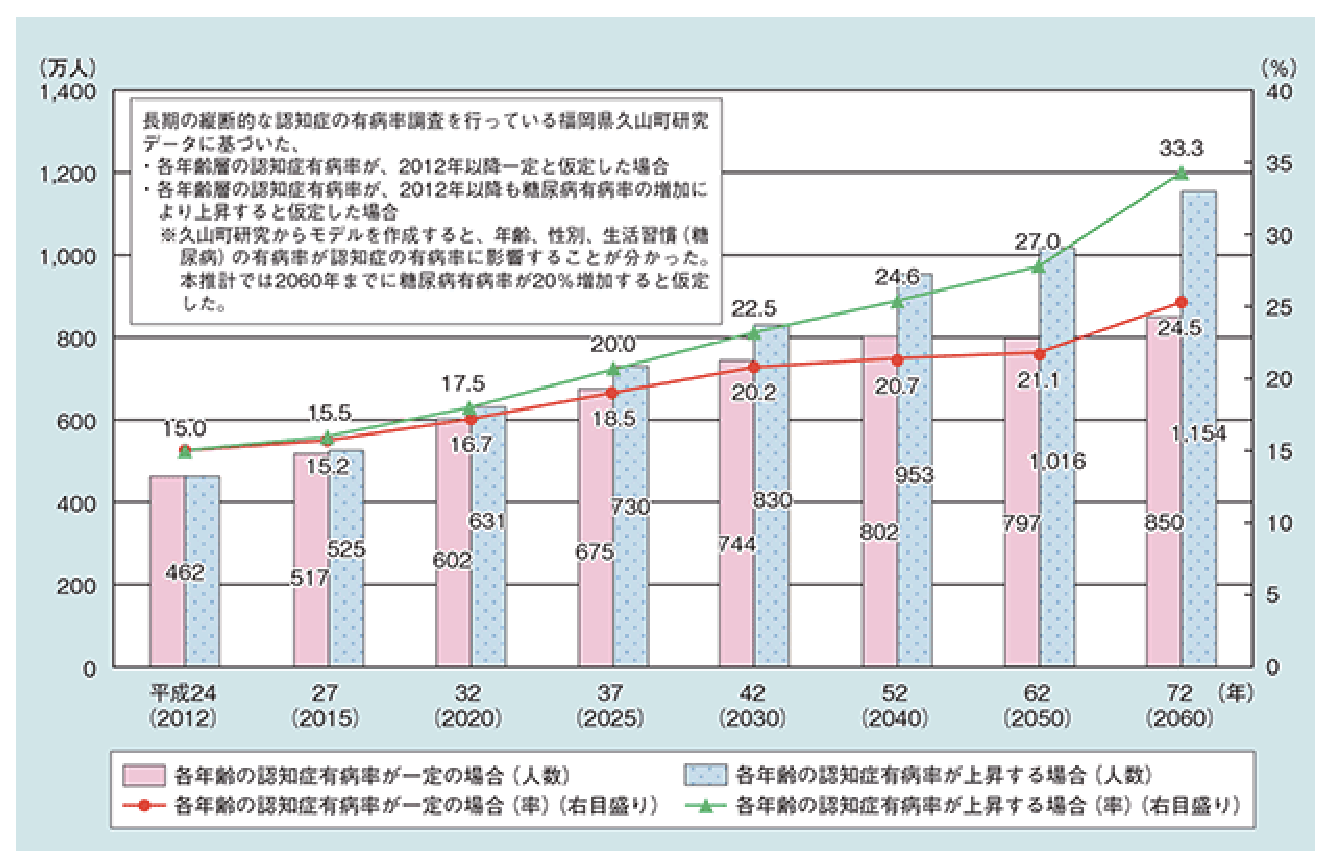
\includegraphics[width=.47\textwidth]{ninchishoukoureishasu.eps}
\caption{認知症高齢者数と有病率の将来推計}
\label{fig:tadou}
\end{center}
\end{figure}

\begin{figure}[tb]
\begin{center}
\includegraphics[width=.47\textwidth]{20171207_cognicise.eps}
\caption{運動教室でのコグニサイズの実施の様子}
\label{fig:HMD}
\end{center}
\end{figure}

\begin{figure}[tb]
\begin{center}
\includegraphics[width=.47\textwidth]{cognistep.eps}
\caption{コグニステップの実施方法(文献[9]より引用)}
\label{fig:HMD}
\end{center}
\end{figure}

\begin{figure}[tb]
\begin{center}
\includegraphics[width=.47\textwidth]{system.eps}
\caption{システム構成図}
\label{fig:HMD}
\end{center}
\end{figure}

\begin{figure}[tb]
\begin{center}
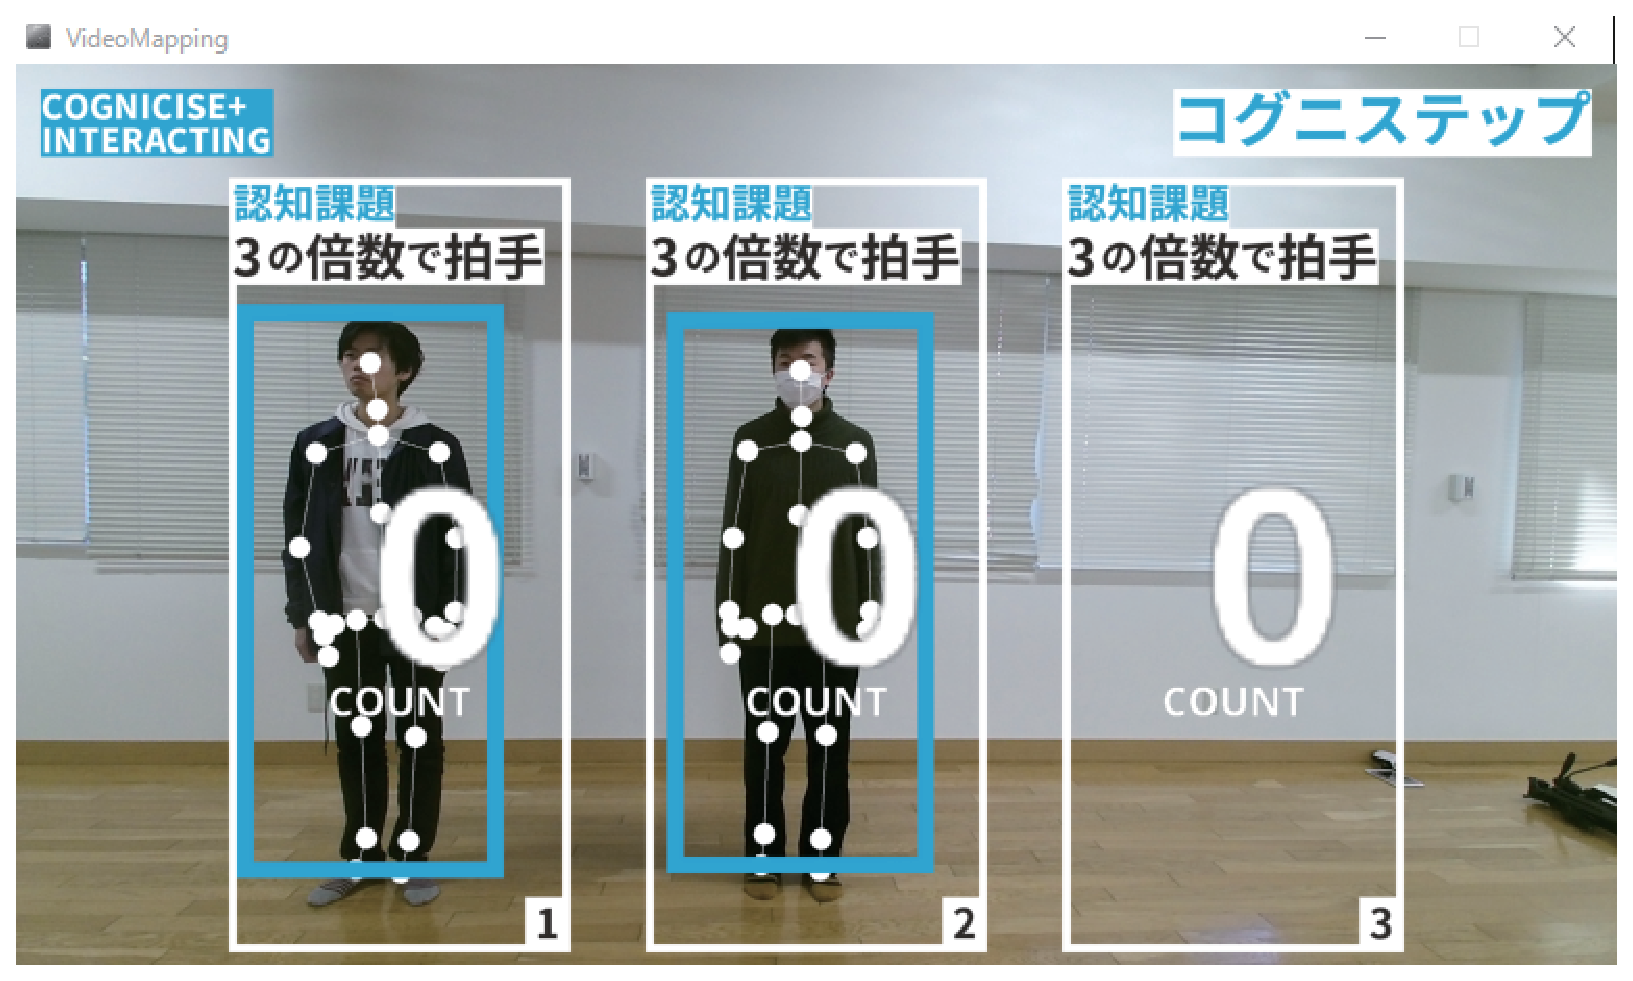
\includegraphics[width=.47\textwidth]{vm_init.eps}
\caption{プロジェクタ投影面}
\label{fig:HMD}
\end{center}
\end{figure}

%--------------------------------------------
\section{提案システム}
本章では,コグニサイズの一つであるコグニステップの認知課題の負荷調整システムについて述べる.提案システムの構成図を図xxに示す.提案システムは全身の身体動作の認識が可能なKinectV2を使用し,認知課題の正誤判定を行う.KinectV2をコグニステップ実施者の対面に設置し,KinectV2に内蔵されるRGBカメラを用いて,コグニステップ実施者を撮影する.プロジェクタを使用し,撮影した動画をコグニステップ実施者の対面に投影する.プロジェクタ投影面には図xxのように,個別に認知課題を表示する.認知課題の正誤判定の集計結果,コグニステップ終了後に認知課題の正答率としてWebサーバ上に保存する.

%--------------------------------------------
\section{実験と考察}
本章では,提案システムを実装し,認知課題の正誤判定の実験を行い,実験結果と考察について述べる.また,高齢者向け運動教室の参加者に対して提案システムを使用した実験を行う.


%--------------------------------------------
\section{まとめ}


%--------------------------------------------

\begin{thebibliography}{9}

\bibitem{}
日本神経学会: ``認知症疾患治療ガイドライン2010''
\bibitem{}
国立長寿医療研究センター: ``認知症予防マニュアル''
\bibitem{}
内閣府: ``平成29年版高齢社会白書''
\bibitem{}
厚生労働省: ``認知症施策推進総合戦略(新オレンジプラン)''
\bibitem{}
島田裕介: ``認知症予防を目的とした運動の効果''
\bibitem{}
重松良祐: ``運動中心の介護予防教室を修了した高齢者のための受け皿事業''
\bibitem{}
国立長寿医療研究センター: ``コグニサイズとは?''
\bibitem{}
国立長寿医療研究センター
\bibitem{}
国立長寿医療研究センター: ``認知症予防へ向けた運動コグニサイズ''
\bibitem{}
滝本幸治: ``地域に根ざした高齢者運動教室の効果検証''

\end{thebibliography}
\end{document}

%%% Local Variables: 
%%% mode: japanese-latex
%%% TeX-master: t
%%% End: 
